\subsection{Udledning af use cases}\label{ssec:usecase}

I samarbejde med Mette, Torben og Anders har vi fundet frem til relevante use cases.

Under det første møde med Mette og Torben blev størstedelen af tiden brugt på at præcisere problemstillingen og prioriteringen af løsningens funktionaliteter.

Heldigvis har førnævnte arbejdsmand Anders Fredensborg været en del af projektgruppen, og vi har derfor haft rig mulighed for at få uddybet tømrernes arbejdsdag.

Use casesne er på "casual form", da der har været begrænset tid, og vi har vurderet, at det ville ikke højne forståelsen ved at lave dem som "fully dressed".\cite{larman}

\subsubsection{Use Cases}

\subparagraph{Registrering af timer}

\textit{Hovedscenarie:} Tidsregistrering af sag der findes.

Tømrer vælger den sag han har arbejdet på. Derefter indtaster han antal timer, han har brugt på hver arbejdstype. Når han har indtastet timer i alt magen til sin timenorm, bliver indtastningen godkendt og han sender timesedlen ind.

\textit{Alternativt scenarier: }

Hvis en tømrer har haft overarbejde denne uge taster han antal timer ind på samme måde som i hovedscenariet.

Hvis en tømrer har arbejdet på en sag, som ikke findes I systemet, vælger han muligheden at oprette en ny sag.
Han indtaster kundeoplysningerne, som er navn og adresse.
Hvorefter han skriver hvad han har lavet og de timer der er brugt.
Tømreren kan vælge at gemme denne sag til senere brug.

Hvis en tømrer har arbejdet på en sag, hvor den specifikke arbejdstype ikke findes, vælger han i stedet at skrive den i det nederste felt betegnet andet.
Tømreren skriver en kommentar i sidefeltet for at fortælle, hvad han specifikt lavede.

Tømreren udfylder sagerne en efter en, når han har indtastet antal timer lig sin timenorm, kan han indsende tidsregistering.

Tømrer skriver sit timeantal som sygdom og ferie, som tilsammen giver sin timenorm.

Tømreren er ansat til 21 timer i ugen, tømreren skriver sit timeantal, som skal give 21 timer i alt.

Tømrer indtaster alle sine arbejdstimer, men mangler at registrere 8 arbejdstimer, da han var syg en dag.
Når han forsøger at indsende tidsregistrering får han besked om, at han mangler at indtaste 8 timer og indsendingen bliver annulleret.

Sekretær vil gerne oprette en ny sag, da de ved, at de skal lave meget arbejde på denne sag i fremtiden.
Hun opretter sagen, og indtaster de nødvendige oplysninger: navn, adresse, evt. telefonnummer og email.

I afsnit \ref{businessmodellering} og \ref{softwaremodellering} vil der blive arbejdet videre med denne use case, hvor der arbejdes med hovedscenariet og det alternative scenarie, hvor en sekretær vil oprette en ny sag.

%\begin{figure} \label{fml}
%    \caption{Product backlog}
%    \centering
%        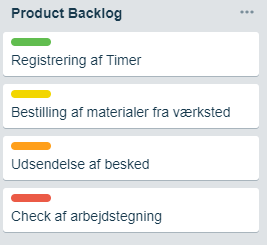
\includegraphics[scale = 1]{ProductBacklog.png}
%\end{figure}

